%% LaTeX2e class for student theses
%% sections/content.tex
%% 
%% Karlsruhe Institute of Technology
%% Institute for Program Structures and Data Organization
%% Chair for Software Design and Quality (SDQ)
%%
%% Dr.-Ing. Erik Burger
%% burger@kit.edu
%%
%% Version 1.3.5, 2020-06-26

\chapter{Introduction}
\label{ch:Introduction}

%% -------------------
%% | Example content |
%% -------------------

Catalysts in combination with chemical reactions are used to speed up a reaction by lowering its activation energy. 
Catalysts increase the reaction rate by lowering the activation energy.
The reaction barrier of a reaction in combination with a catalyst is crucial for its robustness and selectivity.

The catalyst molecules observed in this thesis are derivatives of Vaska's complex, a chemical compound consisting of a variety of different catalysts all with an iridium atom at their center.
The activation barrier depends on the structure of the catalyst and it's ligands.
It varies greatly between different molecules.
Seemingly small changes in the catalysts shape can have a large influence on the catalysts activation barrier [Figure~\ref{fig:struct-diff}].
A rule to predict the activation barrier from the molecules structure cannot easily be found.  
Knowing how to change catalyst molecules in order to lower their activation barrier is a difficult challenge, even to humans.
While the activation barrier can be computed, this process is highly complex and takes a lot of computing power.
This means computing the activation barrier for large datasets of catalysts is currently not feasible.
\begin{figure}[hb!]
  \centering
  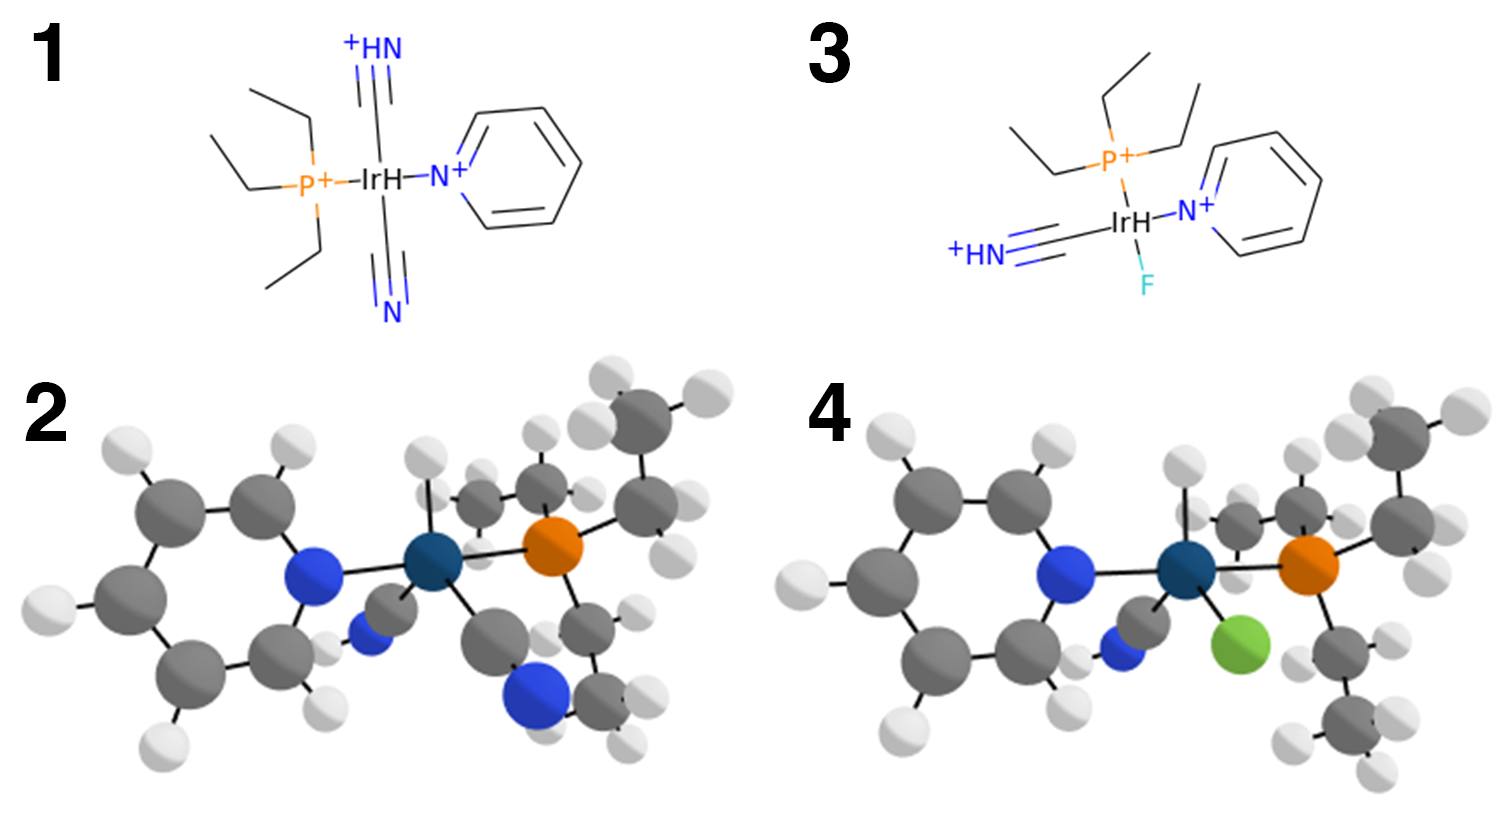
\includegraphics[width=0.8\textwidth]{figures/introduction/elems_intro.png}
  \caption[Example of catalyst molecules]{Two elements with seemingly very similar chemical structures. The chemical structure 1 and it's corresponding 3D structure 2 have an activation barrier of $3.6 kcal/mol$.
  Molecule 3 and it's corresponding 3D structure 4 have an activation barrier of $18.0 kcal/mol$.
  The only difference in the 3D structure of the 2 is the fluorine arm is being replaced by a nitrogen arm.
  The difference is significant considering the distribution of the activation barriers in \ref{fig:barriers}.  }
  \label{fig:struct-diff}
\end{figure}
\\
This Bachelor's thesis explores different approaches to use machine learning to predict the activation barrier of catalyst molecules.
%TODO: Advantages of ML?
Multiple methods of encoding catalyst molecules into machine-understandable formats are proposed.
Using artificial neural networks, the activation barrier is predicted from the catalysts shape.

After being able to predict the activation barrier with high accuracy, different techniques to explain the 
outputs of the neural network are used.
This helps to better understand both the network that is usually regarded as a black box, and the feature space.
The explainers used here are simple gradient based methods, and SHAP explainers \cite{NIPS2017_7062}.
This allows for intuition on which parts of the catalyst molecule contribute to the prediction of the activation barrier.
This intuition may be helpful in further chemical analysis of the metal catalyst.
It might even help the chemist an idea on how a structure needs to be changed in order to lower the activation barrier of the catalyst.
\\

The metal catalysts in question are constructed by combining different ligands around a central Iridium atom.
As illustrated in Figure~\ref{fig:chemspace}, the central atom has multiple locations that allow different types of ligands to be attached to.  
It enables a quick generation of thousands of different catalyst molecules.
By adding more ligands, the dataset can be increased in size with little effort.
For all catalysts in the dataset the activation barrier, along with other properties, is then computed.
\\
As with many machine learning tasks, feature selection is one of the big challenges in this project.
While there are many universal techniques to extract features from chemical structures, they all have their drawbacks.
The feature extracting methods developed in this Bachelor's thesis will rely heavily on the 3D structure of the molecule.
The hypothesis is that the 3D structure is playing an important role in the activation barrier, and encoding the 3D structure will enhance regression accuracy.
Additionally encoding 3D structure will allow to interpretations of the chemical space surrounding the central 
iridium atom to understand the importance of location of the atoms in our molecule.

In order to use feature explainers on the neural network, a reverse mapping from feature space to chemical space needs to be possible.
There currently is no widespread way to encode catalyst molecules that also allows for 
reconstruction of the 3D space and by that an intuition on how the molecule needs to be changed in order ot lower the activation barrier.
Since most chemical feature generators do not specifically focus on catalyst molecules,
but rather provide features for a wide variety of molecules, they generally tend to generate a fully rotational invariant output \cite{Bart_k_2013}.
This full rotational invariance means that information about the location of single atoms is often lost or only implicitly encoded in the features.
Therefore a reconstruction of the molecule only from the features is not possible.
The descriptors proposed here allow to make use of a catalysts special structure.
This enables a partial reconstruction of the 3D shape of the molecule.
In the future this approach could be used to also encode other properties of the molecule.
\\

The seemingly arbitrary distribution of activation barriers among catalyst molecules  was reason to use neural networks for prediction from the generated features.
Neural networks have become the go-to method for high dimensional regression and classification for their ability to adapt well to complex data.
\\
A limitation of neural networks however is their fixed-size input space.
Therefor a representation of the catalyst needs to be found that encodes molecules into a fixed-size set of features.
\\
3D structural encoding comes with its own set of challenges. 
Since a molecules activation barrier it not affected by its rotation or location in space, 
information about rotation and translation should ideally not be part of the molecules features.
\\
In the case of the metal catalysts, achieving translational invariance is trivial.
Since every catalyst is constructed around exactly one metal atom, the molecule can be centered around this metal atom.

For rotational invariance the problem is more complex.
Every catalyst has a reaction pocket attached to its central atom.
In the reaction observed in this thesis, the reaction pocket consists of a single hydrogen atom attached to the central iridium atom.
This reaction pocket has a fixed position that defines the position the reaction will take place.
With the vector from the center of the iridium atom to the center of the reaction pocket, two more degrees of freedom can be removed.
There is no natural way to get rid of the last degree of freedom, rotations around this vector.
%TODO: Figure
Here, 2 different approaches to this last degree of freedom are explored.
The first is using a descriptor that is invariant under rotations around the last degree of freedom.
This removes the need for further normalizations, since all features generated by this descriptor will be invariant.

The second is using data augmentation to teach the neural network about all possible rotations.
This means the molecule is rotated along the last remaining axis of freedom, and multiple examples of the same molecule at different rotations are used as training examples for the neural network.
This ideally allows the network to abstract away the rotation of a molecule.
Using the data augmentation approach, the accuracy of the neural network is significantly higher, reaching a classification error of only  $0.53 kcal/mol$ on a train fraction of 80\%.

After completion of training the networks are able to predict a catalysts activation barrier from its 3D structure.
The main motivation behind encoding the 3D structure is based on the ability to analyse the networks after training.
By analyzing on which features the network is basing its prediction, and translating these features back into 
3D space, an intuition on which parts of the molecule influence its activation barrier can be gained.
Additional information about the influence of different species can be gained 
from separately encoding different atom species into their own set of features.

\section{Dataset}

The dataset used for training and testing contains a total of 1947 samples.
Each sample describes the 3D structure of one catalyst molecule, 
containing the coordinates for every atom in that molecule.
Additional information about the molecule was precomputed among it the reaction barrier focused on in this work [Figure~\ref{fig:barriers}]. %TODO: Reaction barrier for which reaction?
The number of atoms forming one molecule varies between catalysts.
Consistent throughout the dataset is the central iridium atom and the reaction pocket, a single hydrogen atom attached to the center.
The global position and rotation of the molecule within the dataset is arbitrary, and have no effect on its activation barrier.

The dataset was constructed from a set of ligands.
These ligands are placed around the iridium core in a specific order.
There is a total of 3 ligand groups, with every group being able to attach in a different way to the metal center.
By combining different ligands from these groups, catalysts are created [Figure~\ref{fig:chemspace}].

\begin{figure}[H]
  \centering
  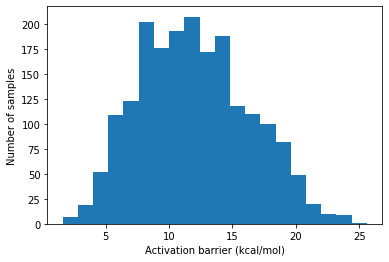
\includegraphics[width=7cm]{figures/introduction/barrier.png}
  \caption[Distribution of activation barriers]{Distribution of the elements activation barrier. The elements have a mean of $11.970 kcal/mol$ and a standart deviation of $4.33 kcal/mol$.}
  \label{fig:barriers}
\end{figure}

Due to this combinatorial approach the dataset could later be increased with relatively low effort.
The biggest hurdle to increasing the dataset size is computing the activation barrier.
This computation is highly complex and therefore not feasible for large datasets.

However, generating a larger dataset without computing the activation barrier could still be helpful when using transfer learning approaches to fine tune the network.
This idea is further discussed in chapter~\ref{ch:Conclusion}.


\section{Previous research}

In previous approaches different machine learning methods were used to predict the activation barrier of the elements in this dataset.
The features extracted from the elements focused on their atomic properties.
However, the features extracted from the molecule did not take into account the spacial structure of the element.
The elements were instead encoded by creating a graph from the chemical structure.
Then elements are grouped by their distance from the metal center.
For each group of elements, features were computed as sum of pairwise products/differences of their atomic properties(such as electronegativity, atomic number, identity, topology and size) \cite{friederich_dos}.


Using these autocorrelation features, a neural network and other forms of regression were used to predict the activation barrier.
Gaussian processes were able to predict the activation barrier within an error of $<1 kcal/mol$ for a train split of $80\%$.

In an unpublished approach, the autocorrelation features were replaced by a graph structure of the molecule.
On this graph structure, a graph convolutional neural network was trained.
When training on a large fraction of the dataset this network reached accuracies 
beyond what could be achieved using autocorrelation features, reaching accuracies of $<0.5 kcal/mol$ for a training fraction of 90\%.

All of these methods used features independent of the 3D structure of the element.
Other than the obvious disadvantage of withholding information from the element, another disadvantage is the lack of interpretability of results.
While these features succeed at predicting reaction barriers, gaining 
information about what part of the molecule is contributing to the prediction is limited or not possible.

\begin{figure}[H]
  \centering
  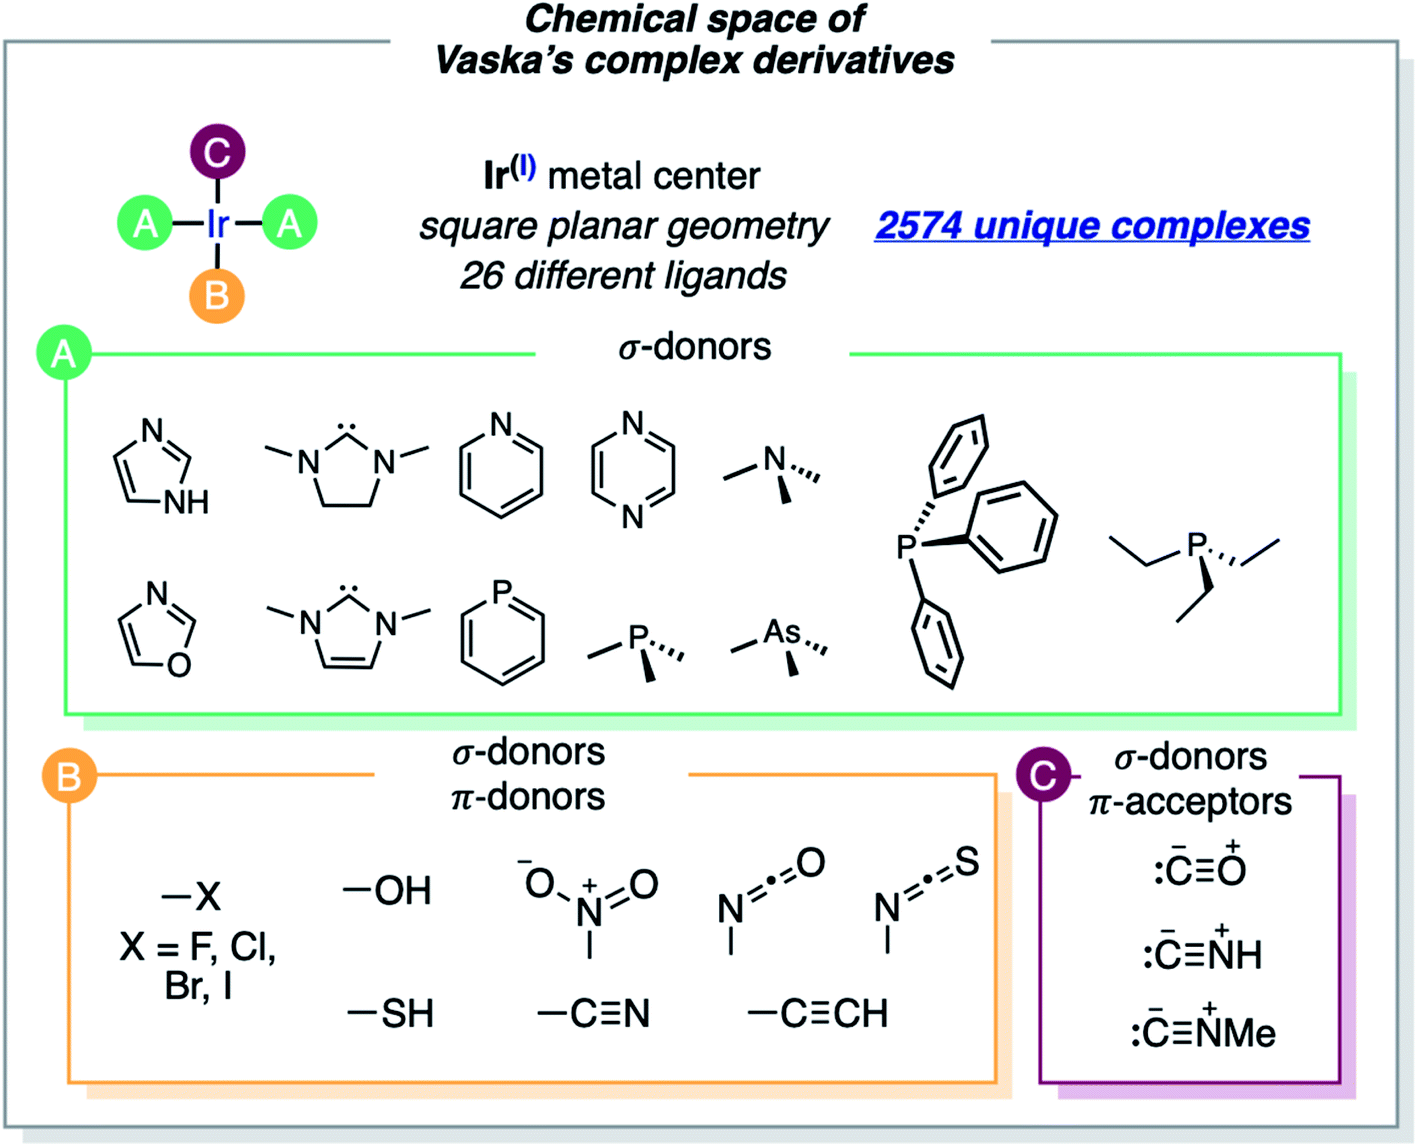
\includegraphics[width=10cm]{figures/introduction/chem-space.png}
  \caption[Vaska's space]{Ligands defining the chemical space associated with Vaska's complex. Reprinted from \cite{friederich_dos}.}
  \label{fig:chemspace}
\end{figure}

The feature extractors introduced in this thesis aim to solve this problem by extracting features that allow for a
partial reconstruction of the chemical space.
This helps to better understand the origin of a prediction and helps to understand the influence of different ligands to the reaction barrier.

Feature extraction is a common problem for machine learning methods in chemical spaces.
Multiple approaches have been proposed for general molecule encoding, 
ranging from encoding properties of molecules, such as the Coulomb Matrix encoder encoding electrostatic interaction of atoms \cite{PhysRevLett.108.058301}
to encoding 3D structures of atomic environments \cite{Bart_k_2013}.

3D structural encoders usually create a fully rotational invariant features.
In the case of SOAP proposed by \citeauthor{Bart_k_2013}, this is achieved by encoding information about the interaction of 
different species rather than encoding the 3D space itself.
Fully invariant 3D descriptors have the advantage of being universally applicable for any kind of molecule, since they have no requirements to the element being encoded.
The drawback being transformations from the features back to 3D space are generally not possible.
In many applications, this is not a problem since the generated features are used only for prediction of an elements properties.
In the applications here the features however should later allow to interpret the 3D space surrounding the molecule and ideally give an idea on how the molecule can be changed to alter its properties.

The idea of using a catalysts special structure for this task, and therefore removing some axes of freedom from the feature space, seems to be an unexplored approach.
\\

Since the structure of the catalyst still leaves 1 degree of freedom, the prediction needs to be partly rotationally invariant.
This is a common problem for neural networks even outside of chemistry.
Generally the approaches to solving these problems can be divided into 2 different groups.

The first being feature engineering to generate features from the data that are fully invariant of rotation.
In point clouds approaches include representing the data as angles and distances rather than the points itself \cite{weiler20183d, 8886052}.
Since these features do not change depending on the rotation and translation of the points, the network does not need to 
abstract away the rotational information of the data.
While this method guarantees full rotational invariance, it requires extensive feature engineering.
Additionally, it may increase complexity of the features and in many cases 
goes hand in hand with the loss of some information from the original dataset. 
Restoring the original data is therefore often impossible.
%The EFD feature generator proposed here implements a fully rotationally invariant description by using 
%descriptor that can be normalized for rotation.

A second approach to rotational invariance is data augmentation.
In image recognition data augmentation has already become the go-to method.
Data augmentation removes the need for extensive feature engineering.
Instead, the training data is augmented along all axes of freedom.
In the case of image recognition, this means rotating, scaling, and in some cases deforming the input images.
By that, the dataset will be filled with more examples for every data point, and ideally the model is able to 
abstract away these features. %TODO: Citation needed
In the case of catalyst molecules, each element will be rotated around the remaining axis of freedom.
The different angles will then be fed into to the network for training.
%The SNAP feature generator proposed here produces a partially rotationally invariant output that needs to be augmented along one axis.
%All the augmentation steps are then fed to the networks in order to teach the network to abstract away the different rotations of the catalyst.

\begin{figure}[H]
  \centering
  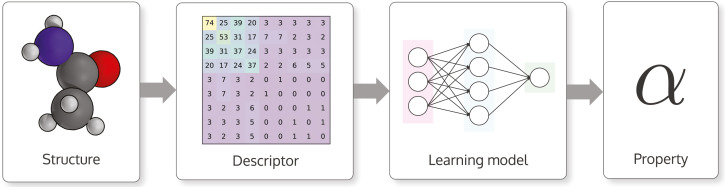
\includegraphics[width=12cm]{figures/introduction/chem-descriptor.jpg}
  \caption[Machine learning in chemistry]{Visualization of feature generation and prediction from the generated features. 
  A fixed size descriptor is generated from the structure. Using machine learning techniques, 
  predictions are made from these features.
  The feature generators proposed here should allow a partial inversion of this process to allow for interpretability of the results.
  Reprinted from \cite{dscribe}.}
  \label{fig:feature-process}
\end{figure}

\section{Objectives}

As with many machine learning tasks, using the raw data as input to machine learning models is not feasible.
Features are therefore generated from the raw data that can be used to learn from.
The typical workflow for machine learning in chemical fields reflects this approach [\ref{fig:feature-process}].

This work can be grouped into 3 main objectives. 
The first is to find a feature extractor that generates features from a catalyst molecule that ideally rotationally invariant.
The second objective is to train a neural network on these features that predicts the activation barrier.
The goal was to achieve accuracy similar or higher to what \citeauthor{friederich_dos} achieved in \cite{friederich_dos}.

In a final step, neural network explainers are used to explain the origin of predictions of the neural networks.
The goal goal is to gain intuition on what parts of the catalyst contribute to the activation barrier, 
and how the catalyst has to be altered in order to lower the activation barrier.


\subsection{Feature generation}

The features should allow a regressor to make predictions from the 3D shape of the molecules.
Therefore features have to be of fixed length for all elements in the dataset.
The amount of atoms in one element cannot influence the number of features.

Ideally the number of features is as low as possible, helping the model to identify the relevant features better.
The number of features cannot be too small as it should still contain all relevant information.
For interpretability of the results, the features should allow for a partial or full reconstruction of the element they are encoding.
This means, given the features, it should be possible to approximate the general shape of the molecule.

To allow for computational exploration of the encoded space, the features should be continuos.
Small changes in the density space should result in small changes in the 
feature space. 
This means hashing from chemical space to feature space is not viable.

Two different approaches to feature generation are prosed.
The first is a fully rotationally invariant output using a rotationally invariant contour description.
While the output of this descriptor is fully invariant, it suffers from sampling issues due to the nature of it's encoding.

The second approach to feature generation was using a combination of basis functions to fully describe a local environment around a central atom.
Using a set of coefficients, the density space surrounding the central atom can be approximated.

\subsection{Regression}

The second step is to predict the activation barrier from these features using an artificial neural network.
A reference for prediction accuracy was set by \cite{friederich_dos}.
The networks proposed here achieve higher accuracy's than the best regression methods proposed in \cite{friederich_dos}.

The regression methods performed on features created with SNAP achieve accuracies $7.22\%$ higher than regression methods on graph convolutions,
the highest accuracy regressors on this dataset to date.

\subsection{Explaining the feature space}
Since the features should allow for an inversion back to the 3D space, it's possible to approximate which areas in 3D space are responsible for the prediction.
Using neural networks explainers, in  a last step the regions in 3D space that influence the regression will be analyzed.
This gives an idea on how different atoms in the dataset influence the prediction.
Looking at the gradient of the input with respect to the activation barrier, an intuition on how the catalyst molecule needs to be 
adapted in order to decrease the activation barrier can be given.
Due to the low resolution of the encoder, the information that can be gained is limited.